\documentclass[smaller,xcolor=dvipsnames]{beamer}
\usetheme[english]{Berlin}
%\usepackage{ngerman}
\usepackage[ngerman]{babel}
\useoutertheme{infolines}
\beamertemplatenavigationsymbolsempty
\setbeamertemplate{caption}[numbered]
\usepackage{pgfplots,tikz,subfigure}
\usepackage{amsmath,amsthm}
\usepackage{hyperref,graphics,graphicx,color,algorithm,algorithmic,enumerate}
\usepackage{mymacros,wrapfig,relsize}
\usepackage{pict2e}
\usepackage[utf8x]{inputenc}
\usepackage{csquotes}

\newcommand{\ri}{\mathrm{i}}
\newcommand{\T}{\mathsf{T}}
\renewcommand{\H}{\mathsf{H}}
\newcommand{\eps}{\varepsilon}
\newcommand{\To}{\rightarrow}
\newcommand{\sddots}{\scalebox{0.6}{$\ddots$}}
\usepackage[pdf]{pstricks}
\usepackage{sansmathfonts}
\usepackage{eurosym}
\usepackage{ulem}
\renewcommand{\O}{\mathcal{O}}
\DeclareMathOperator{\opt}{OPT}
\DeclareMathOperator{\copt}{Compute-OPT}
\DeclareMathOperator{\icopt}{Iterative-Compute-OPT}
\DeclareMathOperator{\ssum}{Subset-Sum}
\newcommand{\opfind}{\text{Find}}
\newcommand{\opunion}{\text{Union}}
\newcommand{\opmakeunionfind}{\text{MakeUnionFind}}
\newcommand{\component}{\text{Component}}
%\usepackage{arev}
%\renewcommand\familydefault{\sfdefault}

\DeclareMathOperator{\loc}{loc}
\DeclareMathOperator{\rank}{rank}
\DeclareMathOperator{\RE}{Re}
\DeclareMathOperator{\IM}{Im}
\DeclareMathOperator{\In}{In}
\DeclareMathOperator{\im}{im}
\DeclareMathOperator{\Gl}{Gl}
\DeclareMathOperator{\spa}{span}
\DeclareMathOperator{\ext}{{ext}}
\DeclareMathOperator{\ind}{ind}
\DeclareMathOperator{\normalrank}{normalrank}
\DeclareMathOperator{\essup}{ess\,sup}
\DeclareMathOperator{\vect}{vec}

\newcommand{\re}{\mathrm{e}}
\newcommand{\ddt}{\tfrac{\mathrm{d}}{\mathrm{d}t}}
\newcommand{\sys}[4]{\left[\begin{array}{c|c} #1 & #2 \\ \hline #3 & #4 \end{array}\right]}

\renewcommand{\tilde}{\widetilde}
\renewcommand{\hat}{\widehat}


\title[]{Optimierung f\"ur Studierende der Informatik}
\subtitle{-- 14. Vorlesung --}
\author[Matthias Voigt]{\textbf{Matthias Voigt$^{1,2}$}}
\institute[]{
\begin{columns}
%\begin{center}
\column{0.45\textwidth}{\centering {$^1$Universit\"at Hamburg \\ Fachbereich Mathematik \\ Hamburg \\ }}
\column{0.45\textwidth}{\centering {$^2$Technische Universit\"at Berlin \\ Institut f\"ur Mathematik \\ Berlin  \\}}
%\end{center}
\end{columns}
}
\date[]{Universit\"at Hamburg
\begin{columns}
\column{0.45\textwidth}{\centering 
\includegraphics[width = 1.2\textwidth]{uhh-logo.png}\\}
\end{columns}
}

\definecolor{tucgreen}{rgb}{0.0,0.5,0.27}
\definecolor{tucred}{rgb}{0.75,0,0}
\definecolor{tucorange}{rgb}{1.0,.5625,0}
\definecolor{mpired}{HTML}{990000}
\definecolor{mpigreen}{HTML}{5C871D}
\definecolor{mpiblue}{HTML}{006AA9}
\definecolor{mpibg1}{HTML}{5D8B8A}
\definecolor{mpibg2}{HTML}{BFDFDE}
\definecolor{mpibg3}{HTML}{A7C1C0}
\definecolor{mpibg4}{HTML}{7DA9A8}
\definecolor{mpigrey}{rgb}{0.9294,0.9294,0.8784}

\newcommand{\Z}{\mathbb{Z}}

\begin{document}

\maketitle

\begin{frame}
\frametitle{Eine zeigerbasierte Datenstruktur für Union-Find}
Die Datenstruktur für diese alternative Implementierung verwendet Zeiger. Jeder Knoten $v \in S$ ist in einem Record gespeichert -- zusammen mit einem dazugehörigen Zeiger, durch den man direkt oder dadurch, dass man weiteren Zeigern folgt, zum Namen der Klasse gelangt, die $v$ enthält\footnote{Falls Sie mit Zeigern wenig vertraut sind: Im vorliegenden Kontext reicht es aus, sich einen Zeiger als einen Verweis auf ein Objekt vorzustellen.}. \\ \medskip

Wie zuvor benutzen wir die Elemente der Menge $S$ als mögliche Namen für die Klassen und betrachten Partitionen, in denen jede Klasse nach einem ihrer Elemente benannt ist. \\ \medskip

Der \alert{Initialisierung} dient die \alert{Operation MakeUnionFind($S$)}, durch die zu jedem $v \in S$ ein Record eingerichtet wird, \alert{in dem $v$ zusammen mit einem Zeiger gespeichert wird, der auf $v$ selbst verweist\footnote{Alternativ könnte man hier den Nullzeiger verwenden.}.} Das bedeutet, dass am Anfang jedes $v$ eine 1-elementige Klasse bildet.
\end{frame}

\begin{frame}
\frametitle{Eine zeigerbasierte Datenstruktur für Union-Find}
Als nächstes betrachten wir die \alert{Union-Operation}: Wir nehmen an, dass $A$ und $B$ zwei verschiedene Klassen sind, die zusammengelegt werden sollen; die Klasse $A$ sei nach dem Knoten $v \in A$ benannt, während die Klasse $B$ nach dem Knoten $u \in B$ benannt sei. \\ \medskip

Es wird dann entweder $u$ oder $v$ als Name für die Vereinigungsmenge gewählt, sagen wir, $v$ sei der Name für die Vereinigungsmenge $A \cup B$. \alert{Dies wird dadurch umgesetzt, dass nichts weiter getan wird, als den Zeiger von $u$ abzuändern:}
\begin{itemize}
\item Der Zeiger von $u$ wird so geändert, dass er nun auf $v$ verweist.
\item Die Zeiger, die zu anderen Elementen von $B$ gehören, werden nicht abgeändert. 
\end{itemize}
Für Elemente $w \in B$, $w \neq u$, bedeutet dies, dass man einer Reihe von Zeigern folgen muss, um den Namen der Klasse zu erfahren, der $w$ angehört: Zunächst wird man dabei zum \enquote{alten Namen} $u$ hingeführt und erst über den Zeiger von $u$ nach $v$ gelangt man zum \enquote{neuen Namen} $v$.
\end{frame}

\begin{frame}
\frametitle{Ein Beispiel}
Zur Illustration anhand eines Beispiels sei $S = \bigl\{ p,q,r,s,t,u,v,w,x,y,z\bigr\}$. Es gebe drei Klassen $\bigl\{s,u,w\bigr\}$, $\bigl\{ p,t,v,z \bigr\}$ und $\bigl\{ q,r,x,y \bigr\}$. Es soll die folgende Situation vorliegen:

\begin{center}
 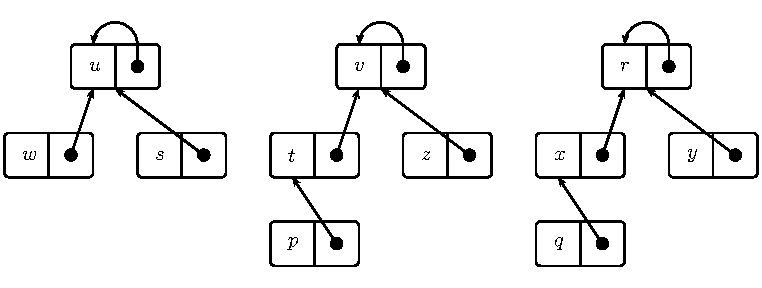
\includegraphics[scale=0.8]{fig104.pdf}
\end{center}

Die drei Mengen dieses Beispiels könnten etwa durch den folgenden Ablauf von $\opunion$-Operationen entstanden sein: $\opunion{(w,u)}$, $\opunion{(s,u)}$, $\opunion{(p,t)}$, $\opunion{(z,v)}$, $\opunion{(t,v)}$, $\opunion{(q,x)}$, $\opunion{(y,r)}$, $\opunion{(x,r)}$.
\end{frame}

\begin{frame}
\frametitle{Ein Beispiel}
Wenn nun als nächste Vereinigung die Operation $\opunion{(v,r)}$ ausgeführt wird, wobei $r$ der Name der durch Vereinigung entstandenen neuen Klasse sein soll, so ergibt sich die folgende Darstellung:

\begin{center}
 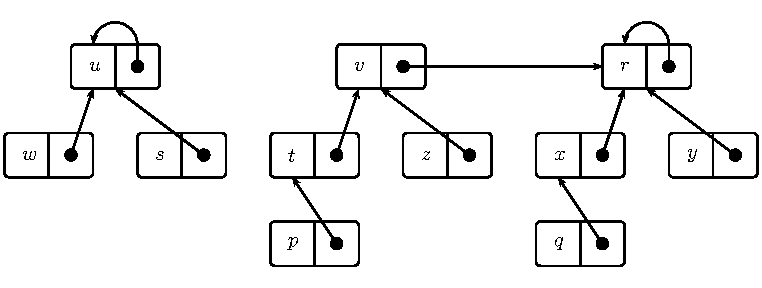
\includegraphics[scale=.8]{fig105.pdf}
\end{center}
\end{frame}

\begin{frame}
\frametitle{Die Union-Operation wird begünstigt}
In dieser zeigerbasierten Datenstruktur ist eine \alert{Union-Operation in $O(1)$ Zeit} durchführbar: 
\begin{center}
 \alert{Man hat nichts weiter zu tun, als einen einzigen Zeiger abzuändern.}
\end{center}
\alert{Die Find-Operation ist dagegen nicht mehr in konstanter Zeit durchführbar}, da wir einer Reihe von Zeigern folgen müssen, um den Namen der Klasse zu erfahren, der ein Element angehört. \\ \medskip

Bevor wir diesen aktuellen Namen mitgeteilt bekommen, durchlaufen wir zunächst die komplette Historie der alten Namen von Klassen, denen das betreffende Element früher einmal angehört hat.
\end{frame}

\begin{frame}
\frametitle{Anzahl der Schritte für eine einzelne Find-Operation}
\alert{Wie viele Schritte benötigt eine einzelne Find-Operation?} \\ \medskip

Die Antwort fällt leicht: Die Anzahl der Schritte, die $\opfind{(u)}$ benötigt, ist gleich der Anzahl der Namen, die die Klasse von $u$ bislang gehabt hat. Ebenso wie bei der Array-Implementierung verfahren wir nach der \alert{Regel, dass bei unterschiedlicher Größe der beiden zu vereinigenden Mengen immer der Name der größeren Menge übernommen wird}. \\ \medskip

\textbf{Man beachte:} Die genannte Regel über die $\opunion$-Operation dient jetzt dazu, die Zeit zu reduzieren, die für eine $\opfind$-Operation aufgewendet werden muss.
\end{frame}

\begin{frame}
\frametitle{Zeitaufwand für ein einzelne Find-Operation}
Die Regel kann dadurch effizient implementiert werden, dass man für jeden Knoten $v$ in dem dazugehörigen Record \alert{ein drittes Datenfeld} einrichtet: \\ \medskip

\alert{Für alle Knoten $v$, die aktuell als Name für eine Klasse dienen, soll in diesem Datenfeld die Größe dieser Klasse gespeichert sein}. Um bei Ausführung einer Union-Operation die Einträge im dritten Datenfeld zu aktualisieren, ist pro $\opunion$-Operation nur eine Addition und nur ein Update nötig.

Unsere Überlegungen laufen auf den folgenden Satz hinaus.
\end{frame}

\begin{frame}
\frametitle{Zeitaufwand für ein einzelne Find-Operation}
\textbf{Satz 2:}
Betrachtet werde die zuvor beschriebene \alert{zeigerbasierte Implementierung der Union-Find-Datenstruktur} für eine Menge $S$ mit $|S|=n$, wobei Vereinigungen den Namen der größeren Menge übernehmen sollen. Eine $\opunion$-Operation benötigt dann $O(1)$ Zeit, $\opmakeunionfind{(S)}$ erfordert $O(n)$ Zeit und eine $\opfind$-Operation nimmt $O(\log{n})$ Zeit in Anspruch. \\ \medskip

\textbf{Beweis}. Die Behauptungen über $\opunion$ und $\opmakeunionfind$ sind leicht zu prüfen: Die Richtigkeit ergibt sich direkt aus der Beschreibung der zeigerbasierten Implementierung. Auch die über die $\opfind$-Operation gemachte Behauptung ist leicht einzusehen: 
\end{frame}

\begin{frame}
\frametitle{Zeitaufwand für ein einzelne Find-Operation}
Die Zeit, die für die Durchführung von $\opfind{(v)}$ für einen Knoten $v$ in einer bestimmten Situation nötig ist, ergibt sich direkt aus der Häufigkeit, mit der der Name der Klasse von $v$ bislang geändert wurde. Da bei Vereinigungen immer der Name der größeren Menge übernommen wird, findet bei jeder Namensänderung der Klasse von $v$ mindestens eine Verdopplung der Klassengröße statt. Da es insgesamt nur $n$ Elemente gibt, kann es demnach höchstens $\log_2{n}$ Namensänderungen der Klasse von $v$ geben. \qquad $\Box$ \\ \medskip
Weitere Verbesserungen durch \enquote{Pfadverkürzung} sind möglich: Dies wird in Skript näher ausgeführt, wobei auf Details verzichtet wird.
\end{frame}

\begin{frame}
\frametitle{Sortieren der Kanten}
Wir wollen die Union-Find-Datenstruktur verwenden, um Kruskals Algorithmus zu implementieren. \\ \medskip

Zunächst haben wir allerdings die Kanten von $G$ in aufsteigender Reihenfolge zu sortieren. Dies geht in $O(m \log m)$ Zeit. Da es zwischen zwei Knoten nur höchstens eine Kante gibt, gilt $m \leq n^2$, woraus man $\log m \leq \log{(n^2)} = 2 \log n$ erhält. Deshalb lässt sich die \alert{Laufzeit für das Sortieren der Kanten} auch angeben als
\[
O(m \log n).
\]
\end{frame}

\begin{frame}
\frametitle{Union und Find}
Nachdem die Kanten sortiert sind, verwenden wir die Union-Find-Datenstruktur, \alert{um die Zusammenhangskomponenten zu verwalten}, die beim schrittweisen Aufbau eines minimalen aufspannenden Baums entstehen. \\ \medskip

Wie wir wissen, geht man die Kanten in aufsteigender Reihenfolge durch. Ist dabei die Kante $e = \{ u,v \}$ an der Reihe, so sind $\opfind{(u)}$ und $\opfind{(v)}$ zu berechnen und zu testen, ob $\opfind{(u)} \neq \opfind{(v)}$ gilt. \\ \medskip

Falls ja, so wird $e$ in den Baum aufgenommen und es hat
\[
\opunion{(\opfind{(u)}, \opfind{(v)})}
\]
zu erfolgen.
\end{frame}

\begin{frame}
\frametitle{Anzahl der Union- und Find-Operationen}
Im Laufe des Kruskal-Algorithmus finden also statt:
\begin{equation*}
\text{$2m$ $\opfind$-Operationen und $n-1$ $\opunion$-Operationen.}
\end{equation*}

Aus Satz 1 für die Array-Implementierung der Union-Find-Datenstruktur bzw. Satz 2 für die zeigerbasierte Implementierung ergibt sich zusammen mit den obigen Anzahlangaben, dass in beiden Fällen
\[
O(m \log n)
\]
eine obere Schranke für die Zeit ist, die im Algorithmus von Kruskal für die $\opunion$- und $\opfind$-Operationen aufgewendet wird.

\end{frame}

\begin{frame}
\frametitle{Laufzeit von Kruskals Algorithmus}
Man kann für die zeigerbasierte Union-Find-Datenstruktur durch Pfadverkürzung noch bessere Laufzeiten für die $\opfind$-Operation herausholen -- für den Algorithmus von Kruskal bringt das jedoch keine Verbesserung der Gesamtlaufzeit: Die Laufzeit des Algorithmus von Kruskal wird unabänderlich durch den Term $O(m \log n)$ dominiert, der durch das Sortieren der Kanten ins Spiel kommt. \\ \medskip

Kurz zusammengefasst können wir feststellen: \\ \medskip

\begin{center}
	\alert{Kruskals Algorithmus kann so implementiert werden, dass sich für Graphen \\ mit $n$ Knoten und $m$ Kanten die Laufzeit $O(m \log n)$ ergibt.}
\end{center}
\end{frame}

\begin{frame}
\frametitle{Ähnlichkeiten der Algorithmen von Prim und Dijkstra}
Der \alert{Algorithmus von Prim} besitzt große Ähnlichkeit mit dem \alert{Algorithmus von Dijkstra}. (Die Gültigkeitsbeweise dieser beiden Algorithmen sind jedoch sehr unterschiedlich.) \\ \medskip

Um die Ähnlichkeit zu verdeutlichen, wird der Algorithmus von Prim so beschrieben, dass er der Formulierung des Algorithmus von Dijkstra \alert{möglichst nahe kommt}. \\ \medskip

Dabei wird vorausgesetzt, dass der betrachtete Graph $G=(V,E)$ zusammenhängend ist. Der Knoten $s$ (\enquote{Startknoten}, \enquote{Wurzel}) sei vorgegeben.
\end{frame}

\begin{frame}
\frametitle{Prims Algorithmus in Pseudocode}
\begin{center}
	\begin{tabular}{rl}
		\multicolumn{2}{l}{\textbf{Prims Algorithmus für ${(G, c, s)}$}} \\
		(1) & Sei $T$ ein Baum in $G$ und sei $S$ die Knotenmenge von $T$. \\
		(2) & Für jedes $u \in V$, speichere einen Wert $d(u)$ und, falls $u \neq s$ und  \\
		    & \qquad $d(u) \neq \infty$, speichere einen Knoten $\operatorname{pred}(u) \in S$. \\
		(3) & Anfänglich sei $T$ der Baum mit der Knotenmenge $S = \{ s \}$ \\ & \qquad und sei $d(s)=0$. \\
		(4) & Für jedes $u \neq s$ sei $d(u) = c(\{s,u\})$ falls $\{s,u\}\in E$ und andernfalls \\ & \qquad $d(u)=\infty$. \\
		(5) & Sei $\operatorname{pred}(u) = s$ für alle $u$ mit $\{ s,u \} \in E$. \\
		(6) & \textbf{while} $S \neq V$ \\
		(7) & \qquad Wähle einen Knoten $v \in V \setminus S$ mit $d(v) = \min{\bigl\{ d(u) : u \in V \setminus S \bigr\}}$. \\
		(8) & \qquad Füge $v$ zu $S$ hinzu und füge die Kante $\{ v, \operatorname{pred}(v) \}$ zu $T$ hinzu. \\
		(9) & \qquad Für jedes $u \in V \setminus S$ mit $\{v,u\} \in E$ und $c(\{ v,u \}) < d(u)$, \\
		    & \qquad\qquad sei $d(u) = c(\{ v,u \})$ und $\operatorname{pred}(u)=v$. \\
		(10)& \textbf{end while}
	\end{tabular}
\end{center}
\end{frame}

\begin{frame}
\frametitle{Laufzeit von Prims Algorithmus}
Aufgrund der Ähnlichkeit zum Algorithmus von Dijkstra ergeben sich Feststellungen zur Laufzeit, die wir auf ähnliche Art für den Algorithmus von Dijkstra getroffen haben:
\begin{itemize}
	\item Die Laufzeit für die beschriebene Version des Algorithmus von Prim ist $O(n^2)$ für $n=|V|$, da die While-Schleife $n-1$ mal durchlaufen wird und die Zeilen (7)--(9) offenbar in $O(n)$ Zeit ausgeführt werden können.
	\item Mithilfe einer Prioritätswarteschlange lässt sich die Laufzeit $O(m \log n)$ erzielen, was beispielsweise für Graphen mit $m = \Theta(n)$ eine Verbesserung gegenüber der Laufzeitschranke $O(n^2)$ bedeutet.
\end{itemize}
Genauer gilt sowohl für Dijkstra als auch für Prim: \alert{Die genannte Laufzeit $O(m \log n)$ ergibt sich, wenn die Prioritätswarteschlange mittels eines Binärheaps implementiert wird (vgl. Kleinberg/Tardos)}.
\end{frame}

\begin{frame}
\frametitle{Laufzeit von Prims Algorithmus}
Wie im Fall von Kruskals Algorithmus können wir also zusammengefasst feststellen:

\begin{center}
	\alert{Prims Algorithmus kann so implementiert werden, dass sich für Graphen mit $n$ Knoten und $m$ Kanten die Laufzeit $O(m \log n)$ ergibt.}
\end{center}
\end{frame}

\end{document}
